% Innehållet i Vasungavisor 2018
%
% Kapitel "I Högan Nord"

\begin{intersong}
\sffamily\bfseries\LARGE\centering{Kun Botnialle Sisään Astuu}
\begin{center}
\includegraphics[width=5cm]{../bilder/ostrobotnia.jpg} 
\end{center}
\end{intersong}
\sclearpage
% Innehållet i Vasungavisor 2018

\beginsong{Festmarsch för Vasa nation}[
	by={Lars Huldén},
	sr={Fritiof Anderssons Paradmarsch},
	index={Från slätterna och havet}] 

\beginverse*
Från slätterna och havet har vi flyttat söderut.
Det gick för att det måste gå.
Nej, om vi här kysser marken!
Vi skrubbar oss i hjärnorna med lärdomens lut.
Men om vi vill
flaxar vi till
och flyger opp åt Kvarken.
Och inte ids vi buga oss för allt som kallas fint.
Vi klampar i salongerna, men klampar genuint.
Vi är en hop som häckar här
i söder några år.
Lever på lån
långt hemifrån
tills graden blivit vår.
\endverse

\beginverse*
Från slätten har vi med oss ner ett eget ögonmått.
Det siktar vi på världen med,
inte blir man imponerad!
Det finns så mycket stort som när det mäts blir ganska
smått.
Hej, om du vill
klämmer vi till
så du blir rent chockerad.
Men inte skall ni buga er som står här runt omkring
för också en som inte är en vasung är nånting.
Här kommer vi långt norrifrån
och är såna vi är.
Men om vi ser
noga på er
så är ni folk ni med.
\endverse

\beginverse*
Och sen så går det kanske som det ofta brukar gå:
Vi stannar här till livets slut.
Men inte glömmer vi marken
och stränderna och skogen där som barn vi härat på.
Nej, om vi vill
så slår vi till
och flyttar opp åt Kvarken.
Och nog för att vi inser att vi inte skiljer oss
så mycket ifrån andra, men det är en sak förstås:
Vi har ett hav, vi har en slätt
som stannat i vår blick.
Stannat hos dig,
stannat hos mig
vart vi i världen gick.
\endverse
\endsong

\sclearpage
% Innehållet i Vasungavisor 2018

\beginsong{Sången om Vasungaflickan}[
	by={Sture Björk},
	sr={Du ska få min gamla cykel},
	index={Först i början rena skräcken},
	]

\beginverse*
Först i början rena skräcken plåga mig,
på nationen gå, det vågar jag nog ej
men tog mod till mig, steg in,
och titta varligt mig omkring.
Usch, vad här är rökigt, skrikigt, stoj och spring.
\endverse

\beginverse*
Det var rätt som mamma sade då jag for,
håll dig borta från nationen, minns din bror.
Hur det gick för honom
efter åtta år i huvudstan,
efter troget vridande på ölfatskran.
\endverse

\beginverse*
Jag skall bara vara flitig, läsa hårt.
Att studera är nog säkert riktigt svårt,
men i kväll kan jag ju stanna här en stund
och dricka te.
Är den tavlan faktiskt så där hemskt på sne'.
\endverse

\beginverse*
Och för pojkar skall jag noga akta mig,
man vet aldrig, hur dom riktigt uppför sig.
Mamma varna' ju mig extra
för att häftigt bliva kär.
Oh, vad han är stilig, han som sitter där!
\endverse

\beginverse*
Men vem fan har sagt att mamma sku ha rätt.
Jag får leva på mitt eget lilla sätt.
Studierna, de får vänta ännu ett år, kanske två,
på nationen vill jag mycket hellre gå!
\endverse

\textnote{Sången sponsoreras av Vasa nations kurator 2016-2018 Frida Forsblom-Prittinen.}

\endsong
\sclearpage
% Innehållet i Vasungavisor 2018

\beginsong{Kun veikot kaupungilla harhaan}[
	by={Risto Vuorijoki 1932},
	sr={},
	index={Talon laulu}]

\beginverse*
Kun, veikot, kaupungilla harhaan
ja olen synkkä, seuraton,
mä silloin tiedän paikan parhaan,
se Ostrobotniamme on.
\endverse

\beginverse*
Kun Botnialle sisään astuu
ja Alakertaan kurkistaa,
siell' heti kohta kaula kastuu,
ja pakko ompi istahtaa.
\endverse

\beginverse*
Siell' näky tuttu silmää kohtaa
ja lasit yhteen kilahtaa,
siell' posket purppuraisna hohtaa,
ja laulu raikas kajahtaa.
\endverse

\beginverse*
Siis takit pois nyt kiskaiskaamme
on tapa pohjalainen tää,
ja veikot, hei, nyt laulakaamme,
niin että katto tärähtää.
\endverse

\beginverse*
Me emme laulamasta lakkaa
ennen kuin aamu sarastaa,
ei täältä kesken poistutakkaan,
tääll' juodaan kautta Pohjanmaan.
\endverse
\endsong
\sclearpage
% Sångtext till VN:s sångbok 2018.

% Denna fil kan användas som sådan, bara verserna,
% namnen och annan rådata behöver bytas ur fälten.
% Tecknet "%" markerar en kommentar som helt och 
% hållet ignoreras av programmet som läser filen.

\beginsong{Nylands nationshus}[ 		% Börja sången här
	by={},					% Författare
	sr={Byssan lull},					% Melodi
	index={Nylands nationshus har raka ikull}, % Alternativa
	index={Fafa ska sjung}]						% sångnamn
	

\beginverse*						% Börja vers
Nyland nationshus ha raka ikull
vårat he staar tär he staar än.
lnt va vi nöjd me na stsylta na meir
vi skutta ikull heila stsiite!
Fafa ska sjung, 
fafa ska sjung,
fafa ska sjung för tållon siin.
\endverse							% Sluta vers

\endsong							% Sluta sång
\begin{intersong}
	\begin{center}
		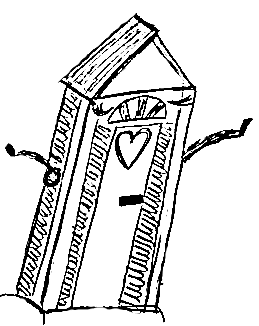
\includegraphics[width=0.5\textwidth]{../bilder/fardigabilder/CamillasFardigaBilder/Nylandsnationshus3.png} 
	\end{center}
\end{intersong}
\sclearpage
% Innehållet i Vasungavisor 2018

\beginsong{Rammens visa}[
	by={Thure Svedlin},
	sr={},
	index={En tärna kom gungande}]

\beginverse*
En tärna kom gungande från Königs bar,
hon gick gnolande Glogatan fram.
På vägen så mötte ett hjältepar,
och den ene var Ferdinand Ramm.
\endverse

\beginverse*
Den andre han var nog en rysk officer
och han hann lite fortare fram.
Så hurra vi alla för Rammens malör
och skåla med Ferdinand Ramm.
\endverse

\beginverse*
Sjörövaren bugar, sjörövaren ler:
"Golubusjka, följ mej nu åt!"
"Nej, förrän jag följer en rysk officer,
så väljer jag Ferdinands stråt."
\endverse

\beginverse*
"Potz tausend Teufel da raube ich dich,
seitjas ti budjesh mojá.
Mon Dieu, eine Herrscherin wirst du für mich,
vot glucklich werden wir da."
\endverse

\beginverse*
Men arg som en spindel framstöter baron
och hejdar på vägen en bil:
"Här skyddar jag dej mot en hel bataljon!"
Sen susa de bort som en pil.
\endverse

\beginverse*
Ja, tärnorna sälja sitt liv så dyrt,
och kampen var midnatt står het.
Men Rammen han segrar - vad sedan sker
är mer än historien vet.
\endverse
\endsong
\sclearpage
{\footnotesize{\bf Ferdinand von Ramm} föddes 1890 i Tavastehus. Han tillhörde en baltisk 
adelssläkt och blev student från Ritter- und Domschule i Reval 1911.
När han i mitten av oktober sammahöst inledde sina studier vid 
Helsingfors universitet valde han att skriva in sig i Vasa nation, 
där han hade släktingar på mödernet, och alltsedan dess förblev han 
vasung och österbottning till själ och hjärta - trots att han knappast 
tillbringade mer än åren under vinter- och fortsättningskriget i 
Österbotten. Rammen berättade själv så här:

``Det var den 9 november 1911 som jag begav mig till
Porthansfesten, iklädd frack och prydd med det röd-gul-svarta
bandet. Mottagandet jag fick var överväldigande vänligt. Man
må ta i betraktande, att jag för herrarna var en helt främmande
figur. Den dåtida inspektorn, prof. Otto Engström, hälsade mig
hjärtligt välkommen, och den kvällen kommer evigt att leva kvar
i mitt minne. Där lärde jag känna kamrater även av finsk
nationalitet, med vilka en trogen vänskap bundit mig genom åren.
Nu började för mig det glada studentlivet inom min egen
korporation. Höstterminen 1911 gick emellertid mot sitt slut.
Terminsavslutningens höjdpunkt bildade julfesten, 'Lilla jul'.
Fastän jag bara var gulnäbb tilldelades jag den stora äran att bli
vald i den kommitté, som fått sig festens arrangemang
anförtrodda, inhandlande av lustiga små presenter m.m. Denna
första julfest i kretsen av mina kamrater kommer alltid att vara
mig oförglömlig. Wasa nation hade på den tiden inget eget 'hem',
utan samlades i Restaurant C. F. Nyberg, belägen mitt emot
'senatsbyggnaden' Som lokal var detta etablissemang egentligen
ganska primitivt, men maten varförträfflig och betjäningen prima.
Många glada sånger sjöngs denna oförglömtiga kväll och först
sent på natten skiljdes man med den glada förhoppningen om
ett återseende under den kommande vårterminen 1912. Var
och en strävade nu hemåt. Ja, jag må säga det var gyllene
tider. Sorglös och glad.''

Ferdinand von Ramm var så genomsyrad av tysk
korporationsanda med dess speciella disciplins- och
hedersbegrepp att han räknade det som sin själfallna plikt att
i början av varje termin personligen anmäla sig hos nationens
kurator och att aldrig försumma ett tillfälle då nationen samlades.
I den mer demokratiska nationen var han en sällsam främmande
fågel med sin spinkiga, något degenererade typ och sin säregna
blandning av gammal fin herrgårdskultur och överdådigt
studentikost festhumör. I hela studentvärlden var han känd och
omåttligt populär, och ännu långt efter det han lämnat studieåren
bakom sig hälsades han med jubelrop var gång han uppenbarade
sig i ett glatt lag på Ostrobotnia. Någon examen avlade han
aldrig, trots grundliga - speciellt historiska - kunskaper och ett
fenomenalt minne. Efter att revolutionen gjort slut på familjens
förmögenhet försörjde han i fortsättningen sig och sin mor på
en enkel kontorstjänst som utrikeskorrespondent hos
andelslaget Labor. Han behärskade sex olika spåk, men inte
finska. Hans ryska var perfekt vilket kom till stor nytta på hans
arbetsplats. Efter kriget sjukpensionerades han och gifte sig
hösten 1947, till sina gamla vänners stora förvåning.

Men ännu när han stod i beråd att med sin hustru bosätta sig i
hennes villa vid Medelhavet för sin återstående livstid,
försummade han inte att komma upp till de äldres samkväm på
Ostrobotnia för att ta farväl av sin nation. Med sviktande
själskrafter erinrade han sig sin ungdoms dårskaper och nertecknade 
dem i en på tyska avfattad relation, som han år
1952 översände till Vasa nation för att förvaras i dess arkiv.
Ferdinand von Ramm avled i Frankrike den 7 december 1960.

Rammens visa skrevs vårvintern 1913 av Thure Svedlin,
nationens kurator 1918-20, till ett spex. Nationens förste kurator
Artur Eklund berättar i dikten ``Ett Königs- minne'', hur han, Svedlin
och Alfred Fahler samlats i det legendäriska ``Gröna rummet'' på
restaurang Karl König vid Mikaelsgatan för att med gemensamma
krafter åstadkomma det spex som skulle bli huvudnumret på ett
allmänt svenskt studentsamkväm. Restaurangens populära bar
kunde under 1910-talet räkna Ferdinand von Ramm bland sina
trognaste stamkunder, vilket förklarar hur han och hans trogne
kumpan Harald ``Mosse'' Monsen, från Nylands nation, dyker
upp för att lyssna till den nyskrivna sången. Sången har länge
funnits med i nationens sångbok, men melodin glömdes under
slutet av sextiotalet, men på initiativ av Sture Björk, en av
nationens mer legendariska sångledare, togs den upp igen i
samband med nationens 75-årsjubileum.}
\ssclearpage




\begin{intersong}
\begin{center}
\includegraphics[width=6cm]{../bilder/rammens_visa.png} 
\end{center}
\end{intersong}
\sclearpage
% Innehållet i Vasungavisor 2018

\beginsong{Ett königsminne}[
	by={Artur Eklund}]

\beginverse*
Där ute rådde klara, skarpa dagen
med brus och oro, jäkt och fåfäng id.
Men nere i vårt källarrum var slagen
en klocka som förkunnat: ingen tid!
\endverse

\beginverse*
Det var ej natt, ty allting var så vaket,
och fråga var ej nu om stängningstid.
Det var ej dag, ty lampan brann i taket,
och fälld gardin höll vakt om rummets frid.
\endverse

\beginverse*
Det var en tid för syner och för drömmar,
för fantasier, hugskott, skämt och skratt.
Det var en tid, som likt en guldflod strömmar
och ger en kvintessens av dag och natt.
\endverse

\beginverse*
Där sutto vi, tre man, som kommit samman
att å en ort från dagens buller ryckt,
uppgöra planer, vårda stämningsflamman
och fånga tankarna i deras flykt.
\endverse

\beginverse*
Att bryta ned var hindrande fördämning
vi togo supar, togo fem och sex.
Här skall, för tusan, snart nog skapas stämning,
här kläckes ut de vasaiters spex.
\endverse

\beginverse*
När glasen lyste av den gula drycken,
då kommo tankarna i brokigt tåg.
I ordens dräkt framträdde många stycken
av dikter, som vårt inre öga såg.
\endverse

\newpage
\beginverse*
Vid instrumentet vällde Djävulssången
med nya ord av skalden Fahler fram.
Vid glasens klang ljöd då för första gången
den sång, vars hjälte är vår vän von Ramm.
\endverse

\beginverse*
Och se! Där kröpo fram så tvenne kunder
av underjordens folk, ett tomtepar.
De kommo gång på gång till korta stunder
och gingo hem ånyo till sin bar.
\endverse

\beginverse*
Och Rammen lyddes hänförd av sin visa.
och varje gång han gick till baren bort,
så var det för att skalderverket prisa
och lämna oss dess vardande rapport.
\endverse

\beginverse*
Och Mosse sedan, liten, torr och mager,
en diable boiteux, en stamkund aven han,
såg drömmande mot fönstrets matta dager,
där dunkla skuggor drevo av och an.
\endverse

\beginverse*
Han blev poetisk, och han hördes tala:
"Hur fjärran ljuder här ej livets brus.
Jag tror, att jag över oss gå böljor svala,
jag tror vi dväljas i Atlantis' hus.
\endverse

\beginverse*
Vi glömts av världen och dess hårda lagar,
vi kommit utom själva livets ström.
Här skiljes ej på nätter och på dagar,
här råder endast sorglös ro och dröm."
\endverse

\beginverse*
Du hade, Mosse, rätt; vi voro alla
den gången sjunkna i Atlantis frid,
men trädde ut ånyo i den kalla
och trista värld vi flytt till någon tid.
\endverse

\newpage
\beginverse*
Men i Atlantis sjönk den dagens minne,
ty se, Atlantis finnes i vår håg.
En ocean förvisso är vårt sinne
och på dess yta föjer våg på våg,
\endverse

\beginverse*
som rastlöst brusande och skumhöljd svalla;
men ned i djupet är det stilla ro
och evigt vita lysa torn och vallar
av sjunken stad, där våra minnen bo.
\endverse
\endsong
\sclearpage


\beginsong{Nikodemos}[
	by={Lars Huldén}] 



\beginverse*
Nikodemos, Nikodemos
var en höglärd man.
Han gick mitt i natten
för att söka katten.
Hem till någon, hem till någon
gick istället han.
\endverse

\beginverse*
När han bulta', när han bulta' 
steg den andre opp.
Knappt han öppnat dörren
åt främlingen förrän
frågor hagla', frågor hagla' 
mot hans huvudknopp.
\endverse

\beginverse*
''Alla vet att, alla vet att
du är pedagog,
en gudabenådad
hos oss aldrig skådad.
Men det andra, men det andra
är väl bara båg?''
\endverse

\beginverse*
Nikodemos, Nikodemos
ville veta mer
om den nya läran,
kom med en begäran:
''Gör ett under, gör ett under!
Tror gör den som ser.''
\endverse

\beginverse*
Men i stället, men i stället
fick han många ord.
Gubben blev besviken;
av metaforiken
kände han sig, kände han sig
platt tillintetgjord,
\endverse

\beginverse*
''Inte kan man, inte kan man
nånsin födas om.
Det förstår väl fler att
är för komplicerat'',
mena' gubben, mena' gubben,
ångra' att han kom.
\endverse

\beginverse*
Vinden viner, vinden viner
och far dit den far.
''Vad är det med det då?
Alla vet det är så!''
Ingivelsens, ingivelsens
virvelvind det var.
\endverse

\beginverse*
Full förklaring, full förklaring
är det svårt att få.
Såvitt man förstår är
allting metaforer,
som får tydas, som får tydas
Det är vackert så.
\endverse

\textnote{Bibelvisa skriven av hedersmedlem Lars Huldén för Vasa nation 29.2.2008 vid kyrkkaffet efter hedersmedlem John Vikströms predikan.}

\endsong

% Innehållet i Vasungavisor 2018

\beginsong{Österbottnisk dryckesvisa} 

\beginverse*
Nu drickom goda vänner, skål gutår!
Nu drickom goda vänner, skål gutår!
/: Närvarande, frånvarande 
och alla vägafarande gutår!:/
\endverse

\vspace{5mm}
\endsong
\sclearpage
% Innehållet i Vasungavisor 2018

\beginsong{Jag är vasung}[
	by={},
	sr={Jag är lapp och jag har mina renar}]

\beginverse*
Jag är vasung och har lite renat
ja, om hembränt så tycker jag bäst
ty att köpa blir dyrt så förbenat
och då saknas ju smaken av jäst!
\endverse

\beginverse*
Här vid foten av snöklädda Pampas
finns en plats dit jag går varje vår
det är faktiskt nåt särskilt med stället
det är där apparaten min står.
\endverse

\beginverse*
Men en natt var det odjur i trakten
där var skära elefanter och möss
så till trolltrummans ljud upptogs jakten
och till kokaren sa jag ajöss.
\endverse

\beginverse*
Men en gång när jag for upp till Pampas
fanns av kokaren inte ett spår
ty se länsman han hittade stället
och i finkan så ensam jag går.
\endverse
\endsong
%% Innehållet i Vasungavisor 2018

\beginsong{Pias snapsvisa}[
	by={Pia Jåfs},
	sr={Smile},
	index={Snaps, den är ljuv och härlig}]

\beginverse*
Snaps, den är ljuv är härlig
och inte alls förfärlig
Av den så njuter vi,
skålar och sjunger.
En snaps den gör livet soligt,
snaps, känn hur allt blir roligt.
Höj nu ditt glas och skåla glatt
och drick sen ur!
\endverse
\endsong
\begin{intersong}
\begin{center}
\includegraphics[width=6cm]{../bilder/kun_veikot.png} 
\end{center}
\end{intersong}
\sclearpage
\sclearpage

\begin{intersong}
\end{intersong}
\input{LauletaanpaMeNuoretPojat.tex}
\sclearpage
%% Innehållet i Vasungavisor 2018

\beginsong{Vi skålar för våra vänner}[
	by={},
	sr={We wish you a merry christmas}]

\beginverse*
Vi skålar för våra vänner,
och dom som vi känner,
och dom som vi inte känner,
dom skiter vi i!
\endverse

\beginverse*
Vi skiter i våra vänner,
och dom som vi känner,
och dom som vi inte känner,
dom skålar vi för!
\endverse

\vspace{5mm}
\endsong
%% Innehållet i Vasungavisor 2018

\beginsong{Pappa kom bort}[
	by={},
	sr={}]

\beginverse*
Pappa kom bort,
när vi var i Köpenhamn.
Så slutar visan.
\endverse
\endsong
%\begin{figure}[!b]
%\begin{center}
%\includegraphics[width=3cm]{../bilder/pappa.jpg} 
%\end{center}
%\end{figure}
%\sclearpage
%% Innehållet i Vasungavisor 2018

\beginsong{Isoo-Antti ja Rannanjärvi}[
	by={},
	sr={}]

\beginverse*
Isoo-Antti ja Rannanjärvi
ne jutteli kahren kesken:
Tapa sinä Kauhavan ruma vallesmanni,
niin minä nain sen komian lesken.
\endverse

\beginverse*
Isoo-Antti oli ensimmäänen
ja Rannanjärvi oli toinen,
Pukkilan Jaska se Kauhavalta
oli kolmas samanmoinen.
\endverse

\beginverse*
Sitten on piru, sano Rannanjärvi,
jos minä miestä pelkän;
tervastampulla kuonon päälle
ja teräksellä pitkin selkää.
\endverse

\beginverse*
Vaasan veri ei vapise,
eikä Kauhavan rauta ruostu;
niskasta kiinni ja puukoolla selkähän,
jonsei se muutoon suostu.
\endverse

\beginverse*
Ensin ne portahat särjettiin
ja sitten vasta muuri;
Isoo-Antti se erellä meni,
joka joukosta oli suurin.
\endverse

\beginverse*
Ei saa laulaa Rannanjärvestä,
Rannanjärvi on kuollu.
Rannanjärven hauralle
on marmorikivi tuotu.
\endverse
\endsong
%\sclearpage